
%\documentclass[reprint,amsmath,amssymb,aps,showpacs,showkeys]{revtex4-1}
\documentclass[reprint,amsmath,amssymb,aps,showpacs,showkeys]{revtex4}


\usepackage{graphicx}
\usepackage{dcolumn}
\usepackage{bm}
\usepackage{amsmath}
\usepackage{xspace}
\usepackage[usenames,dvipsnames,svgnames,table,xspace]{xcolor}


\begin{document}

\newcommand{\fm}{\mbox{fm}}
\newcommand{\MeV}{\mbox{MeV}}
\newcommand{\GeV}{\mbox{GeV}}
\newcommand{\pt}{\ensuremath{p_{T}}\xspace}
\newcommand{\pta}{\ensuremath{p_{T1}}\xspace}
\newcommand{\ptb}{\ensuremath{p_{T2}}\xspace}

\title{Jet Energy Loss at LHC}



\author{Vineet Kumar}
\email{vineetk@barc.gov.in}
\affiliation{Nuclear Physics Division, Bhabha Atomic Research Center, Mumbai, India}

\author{Prashant Shukla}
\affiliation{Nuclear Physics Division, Bhabha Atomic Research Center, Mumbai, India}
\affiliation{Homi Bhabha National Institute, Anushakti Nagar, Mumbai, India}

\date{\today}



\begin{abstract}
  In this work, the jet energy loss is analyzed using a monte carlo method.
  The data from LHC at $\sqrt{s_{\rm NN}}$ = 2.76 TeV and 5.02 TeV is used to extract
  the perameters for specific energy loss of jets inside QGP. Our calculations give
  good discription of the nuclear modification factor and asymmetry measurements at
  LHC.
\end{abstract}

\pacs{12.38.Mh, 24.85.+p, 25.75.-q}
\keywords{quark-gluon plasma, direct photon}

\maketitle

\section{Introduction}
\label{Sec:Introduction}




\section{Jet energy loss}
\label{Sec:JetEnergyLoss}


\begin{figure*}
  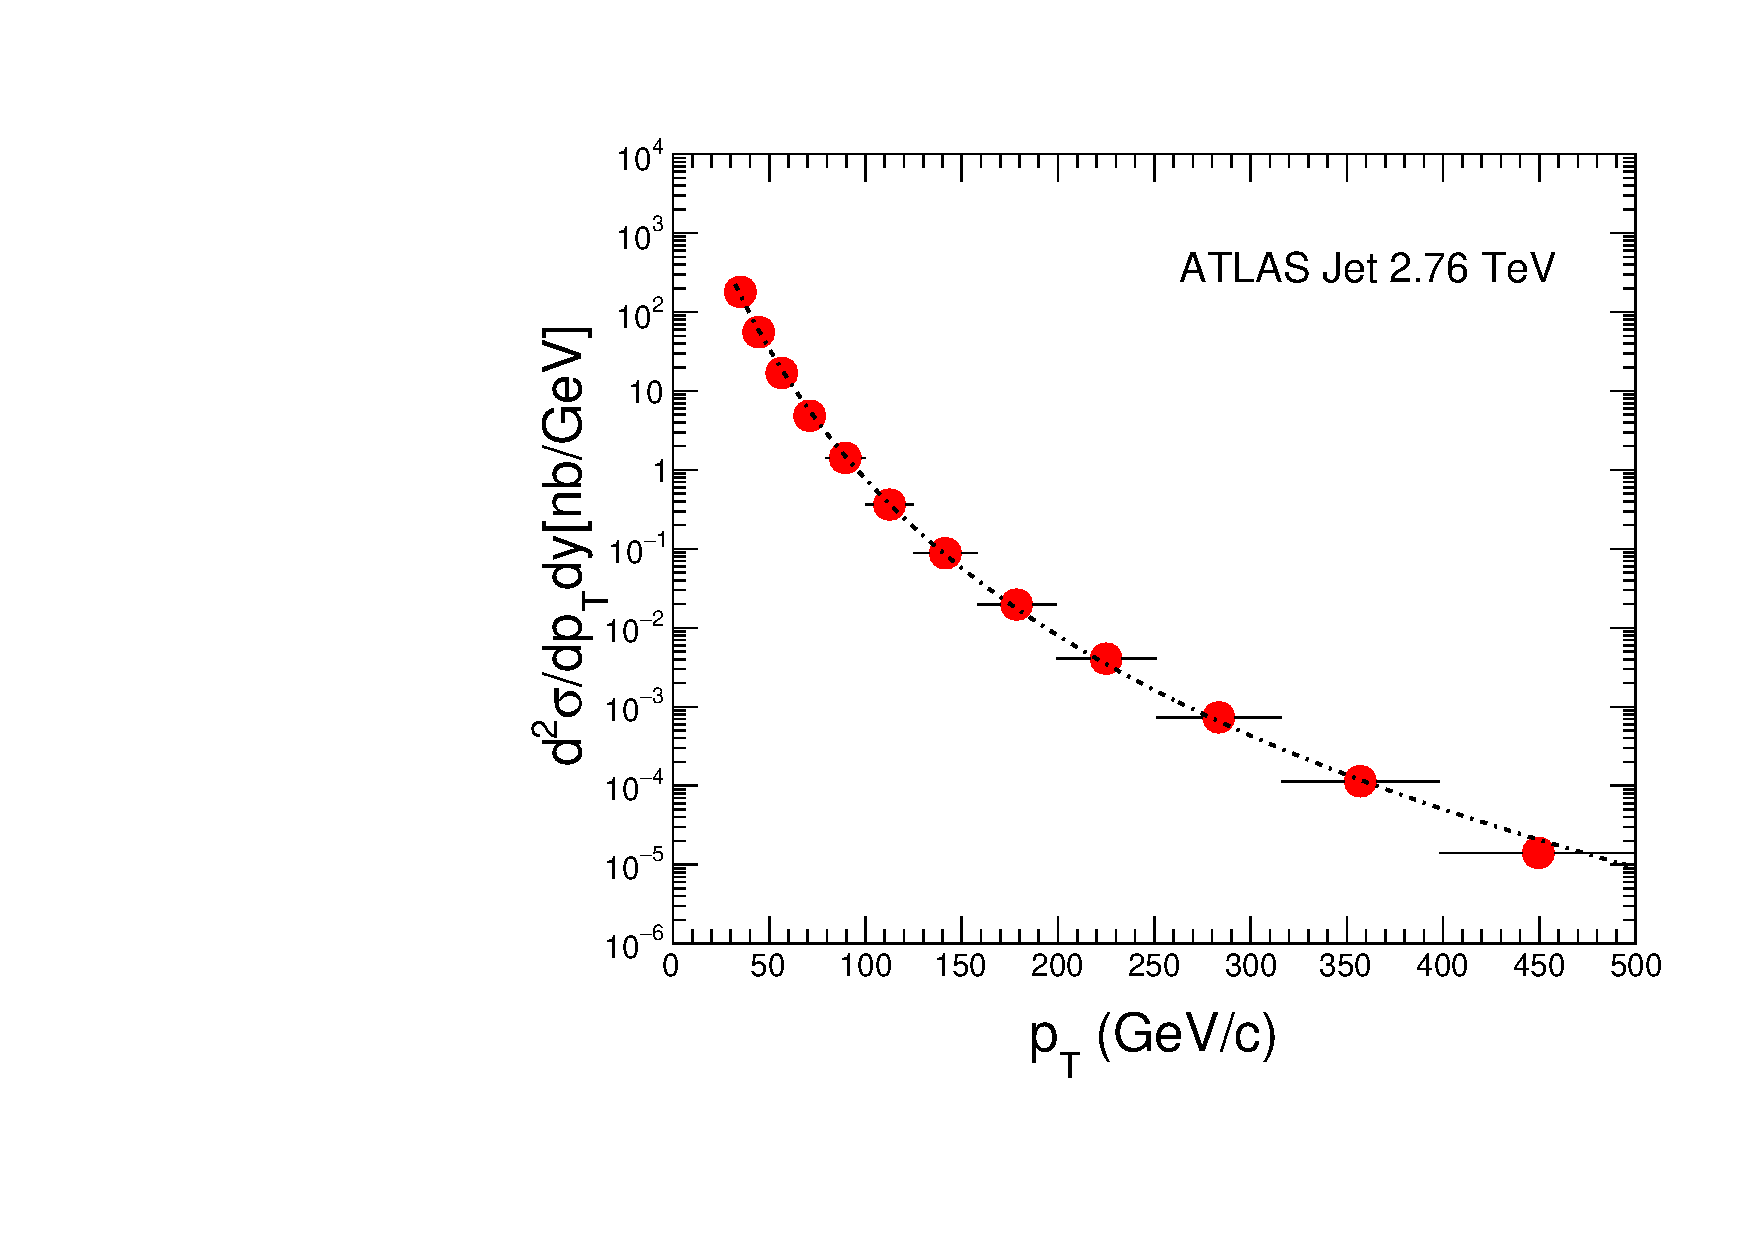
\includegraphics[width=0.49\textwidth]{Figures/Fig_ATLAS_JetYield_JetPt_PP276TeV.pdf}
  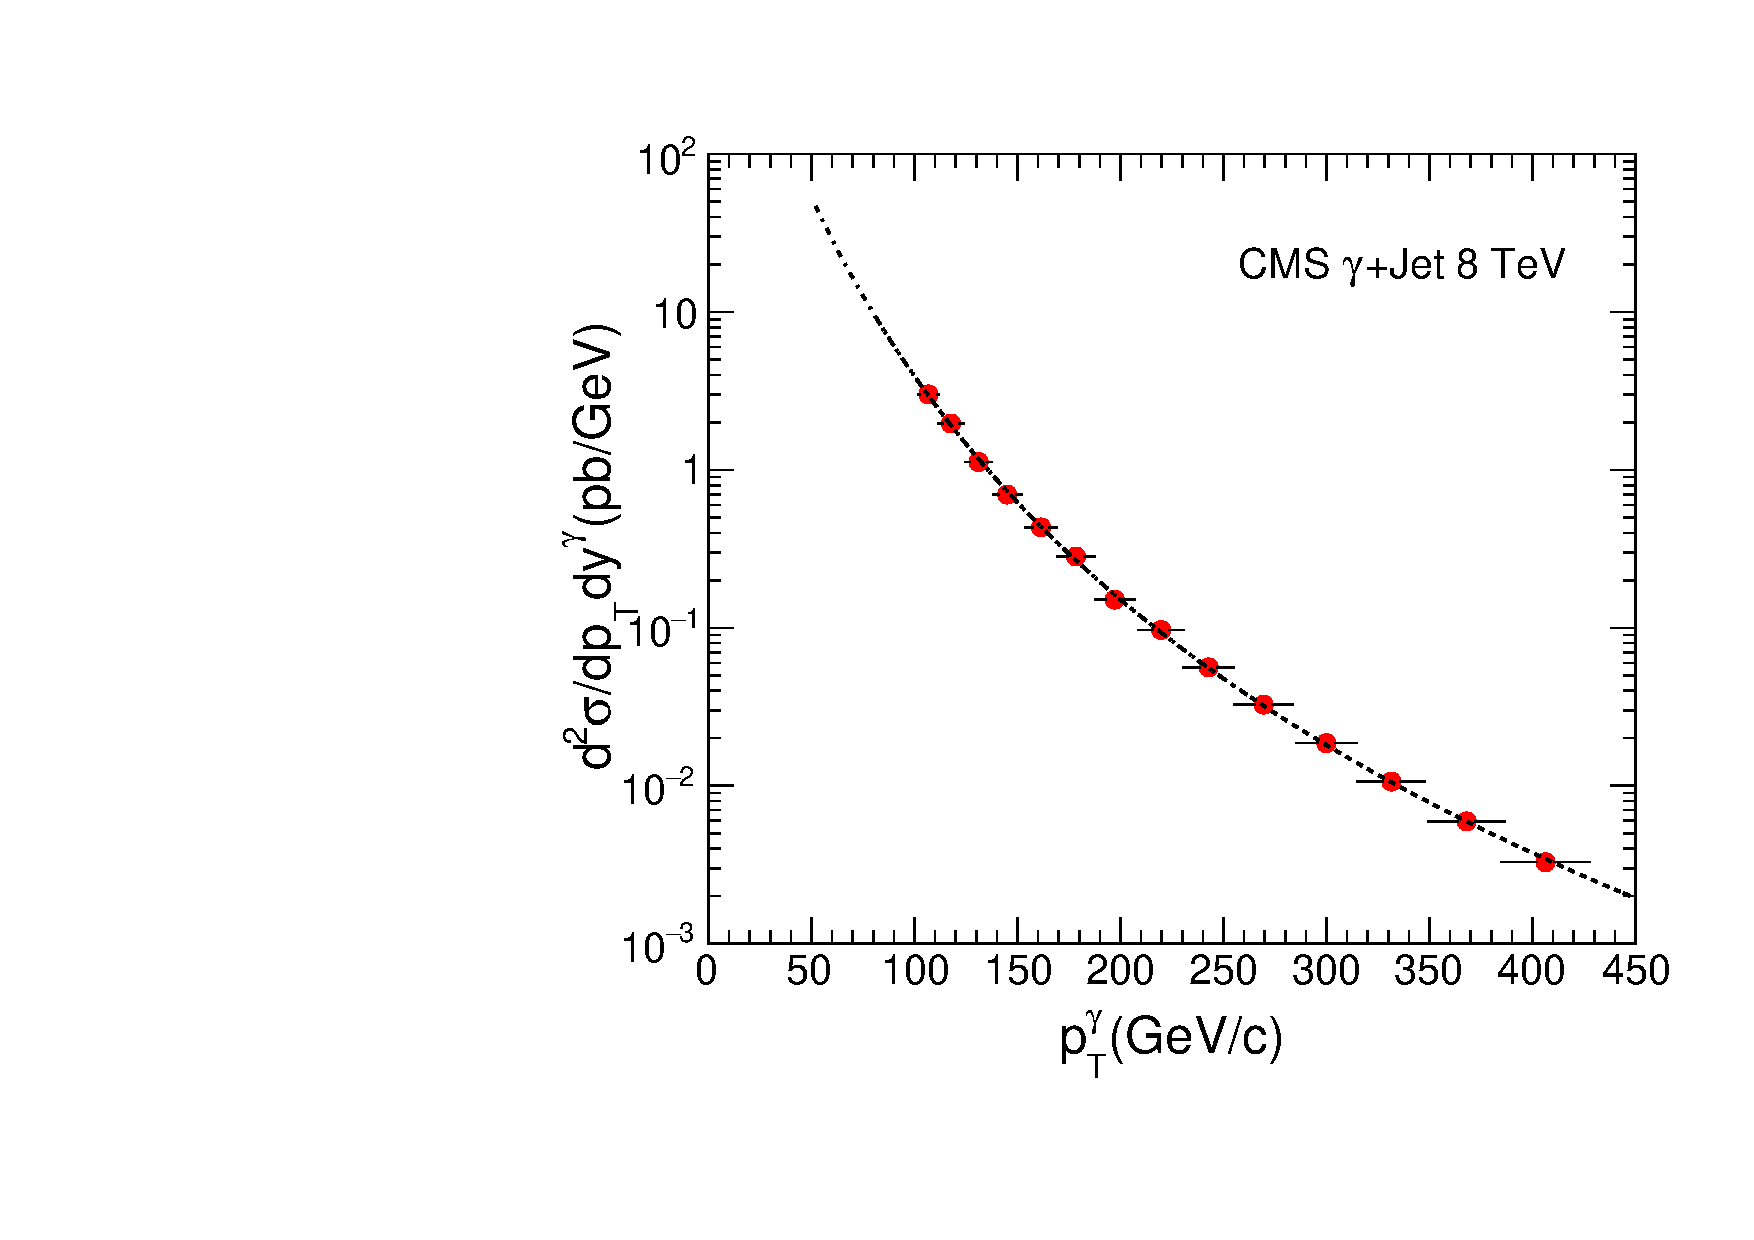
\includegraphics[width=0.49\textwidth]{Figures/Fig_CMS_JetYield_GammaPlusJet_JetPt_PP7TeV.pdf}
  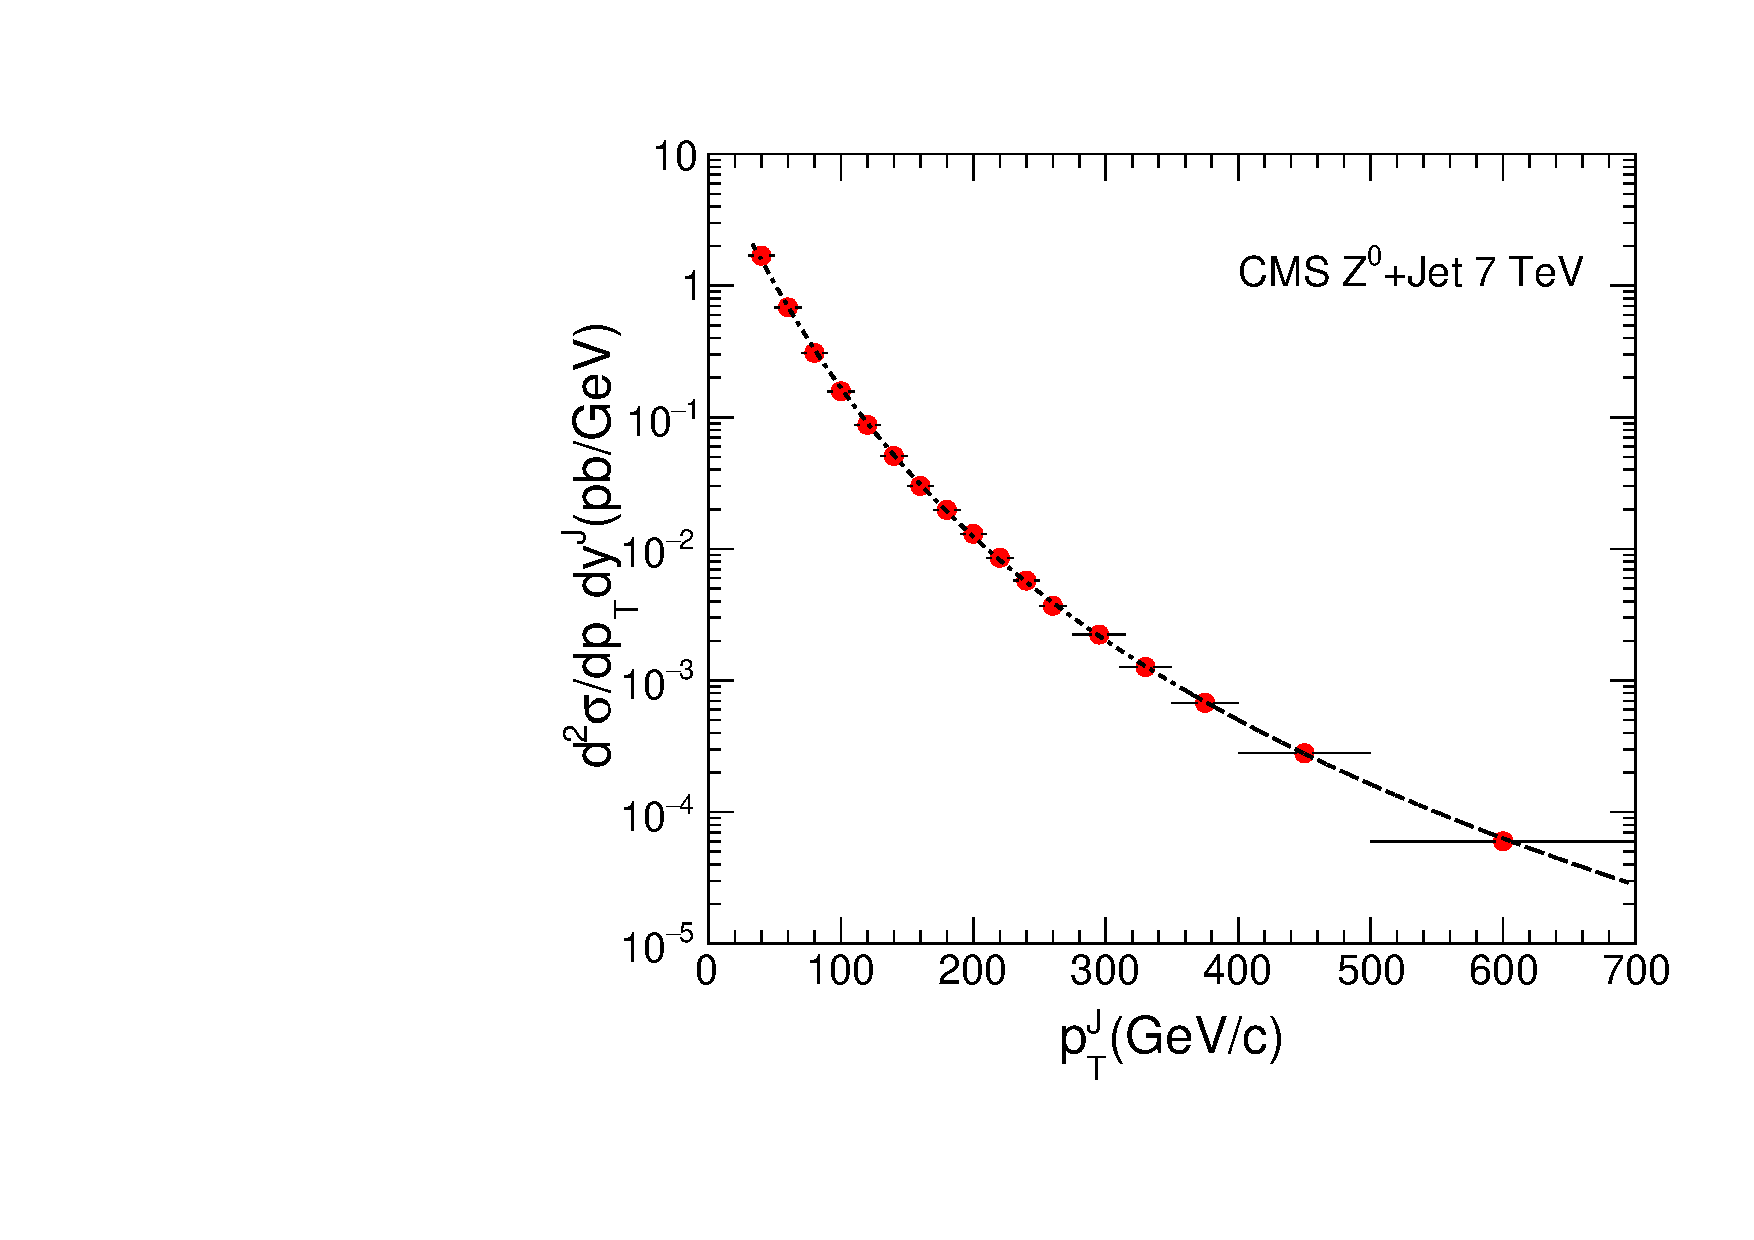
\includegraphics[width=0.49\textwidth]{Figures/Fig_CMS_JetYield_Z0PlusJet_JetPt_PP7TeV.pdf}
  \caption{(Color online) Jet yields as a function of jet \pt measured by ATLAS and CMS experiments.
    These yields are used in our calculations to generate the pp spectrum.}
  \label{Fig:DiJetAsymPt}
\end{figure*}


The Jet \pt distribution in pp collisions is measured by CMS and ATLAS experiments at LHC.
We fit the jet \pt distribution with Hegedorn function.

\begin{equation}
  f(\pt) = \frac{dn}{dy}(1+\frac{\pt}{p_0})^{-n}\\
\end{equation}

The Jet \pt is generated from the fitted function. Now the QGP medium is assumed as a
static sphere. The radius of the medium is related to the centrality of the collision
as 
\begin{equation}
  R = R_{A}\sqrt{\frac{\rm N_{part}}{2A_{m}}}\\
\end{equation}

here $R_{A}$ and $A_{m}$ are the radius and Atomic mass of the Pb nucleus. The
N$_{\rm Part}$ is the number of participant in that particular collison class.

The cordinate $r$ and $\phi$ are then generated randomly. The maximum value of the
cordiante $r$ is the radius $R$ of the system formed. We assume that both partons
move back to back before fragmenting to jets. 


\begin{figure*}
  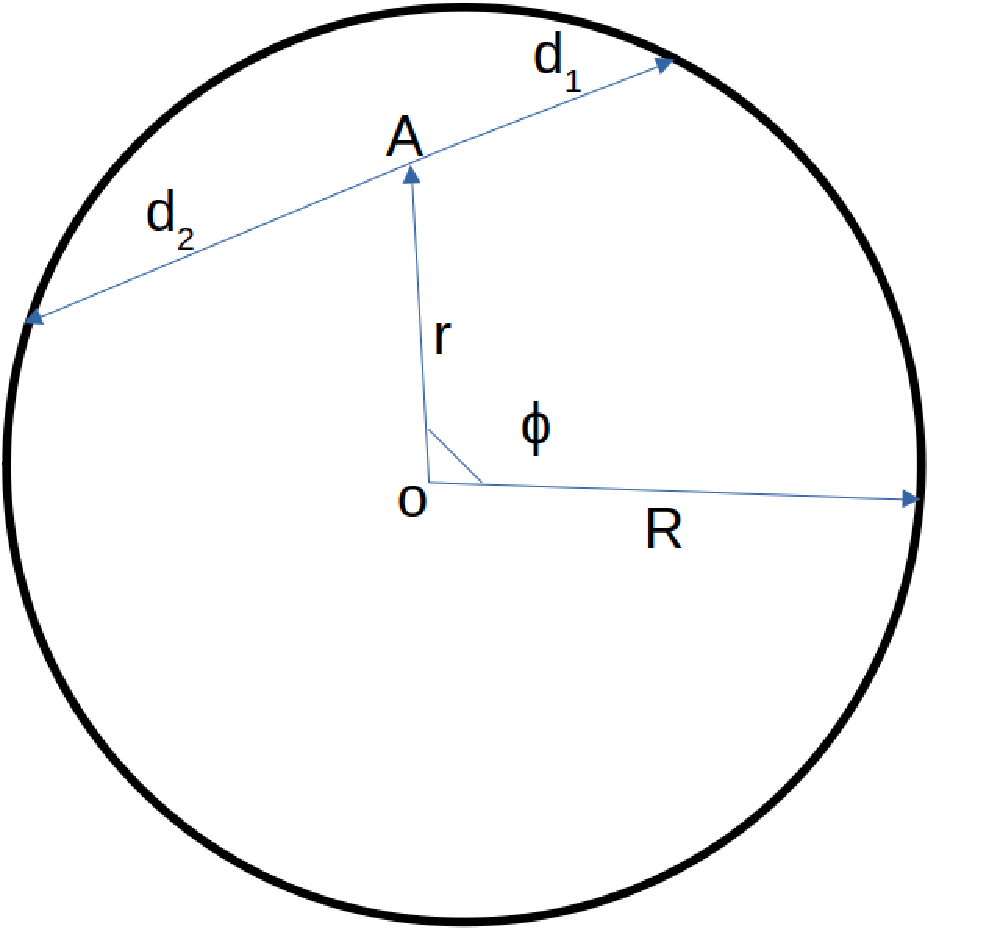
\includegraphics[width=0.49\textwidth]{Figures/DiJetDia.pdf}
  \caption{(Color online) Figure showing the diagram of a diJet system.}
  \label{Fig:DiJetDiagram}
\end{figure*}

The pathlenghts $d_{1}$ and $d_{2}$ can be calculated as follows
\begin{eqnarray}
  d_{1} &= &\sqrt{R^{2}-r^{2}~sin(\phi)} - r~cos(\phi) \nonumber \\  
  d_{2} &= &\sqrt{R^{2}-r^{2}~sin(\pi+\phi)} - r~cos(\pi+\phi)  
\end{eqnarray}

The specific energy loss (energy loss per unit length), dE/dx have following
relation with the \pt of jet

\begin{equation}
  \frac{dE}{dx} = M \pt^{\alpha}\\
\end{equation}

Here M and $\alpha$ are two parameters. We want to constrain these parameters with the
help of LHC measurements and see their variations as a function of collision centrality
and per nucleon energy.

The total energy loss for a jet then can be calculated as

\begin{equation}
  \Delta E = \frac{dE}{dx} \times d \\
\end{equation}
 where $d$ is the pathlenght of the jet inside the medium.
 If $\Delta E_1$ and $\Delta E_2$ are the energy loss for both the jets
 respectively we can get the final jet energies as

 \begin{eqnarray}
   \pta &= & \pt - \Delta E_1 \nonumber \\
   \ptb &= & \pt - \Delta E_2 \nonumber   
 \end{eqnarray}

 and the Jet asymmetry can finally be calculated as

\begin{equation}
  A_{J} = \frac{\pta-\ptb}{\pta+\ptb} \\
\end{equation}
 


 
 


\begin{figure*}
  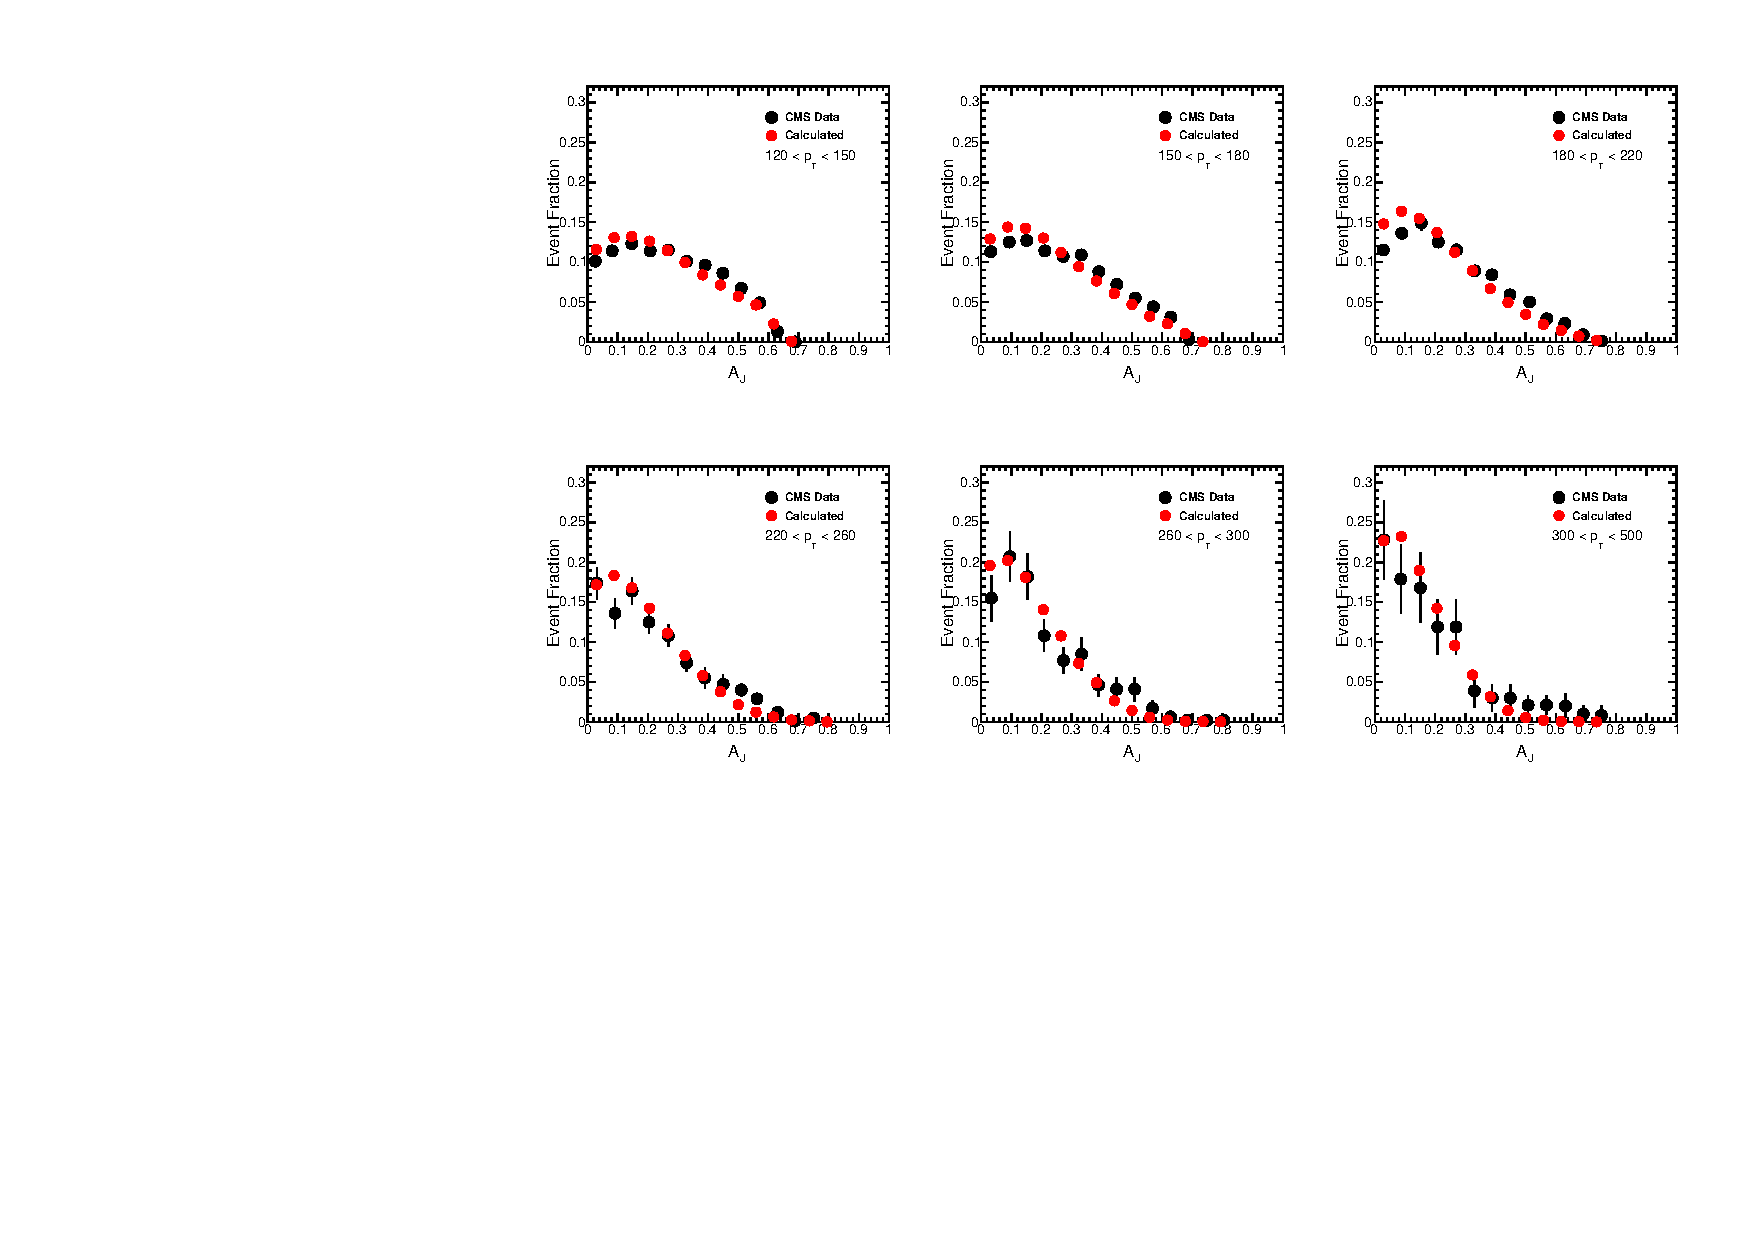
\includegraphics[width=0.99\textwidth]{Figures/Fig_Asym_DiJet_Pt.pdf}
  \caption{(Color online) DiJet asymmatry as a function of jet \pt measured by CMS experiment
    compared with our calculations.}
  \label{Fig:DiJetAsymPt}
\end{figure*}



\begin{figure*}
  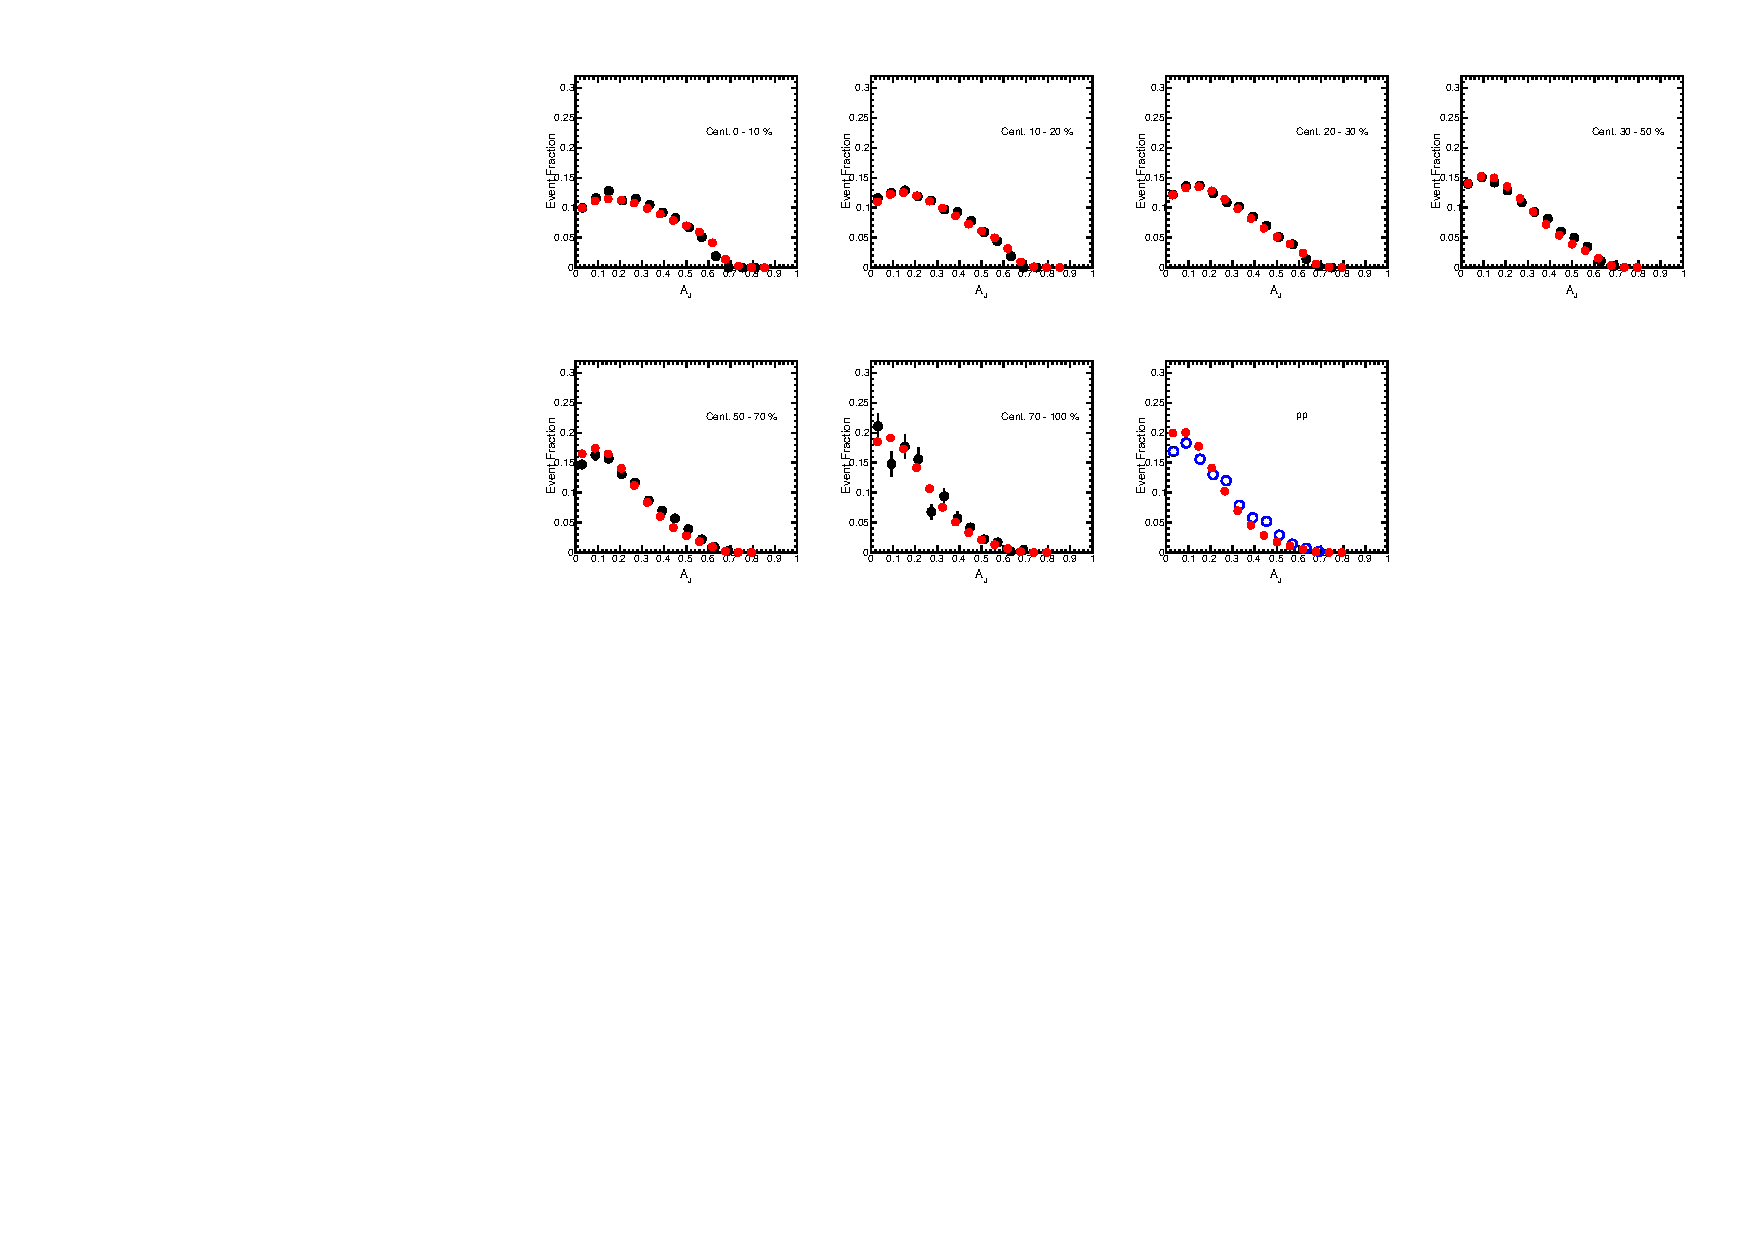
\includegraphics[width=0.99\textwidth]{Figures/Fig_Asym_DiJet_Centrality.pdf}
  \caption{(Color online) DiJet asymmatry as a function of collision centrality
    measured by CMS compared with our calculations.}
  \label{Fig:DiJetAsymCent}
\end{figure*}



\begin{figure*}
  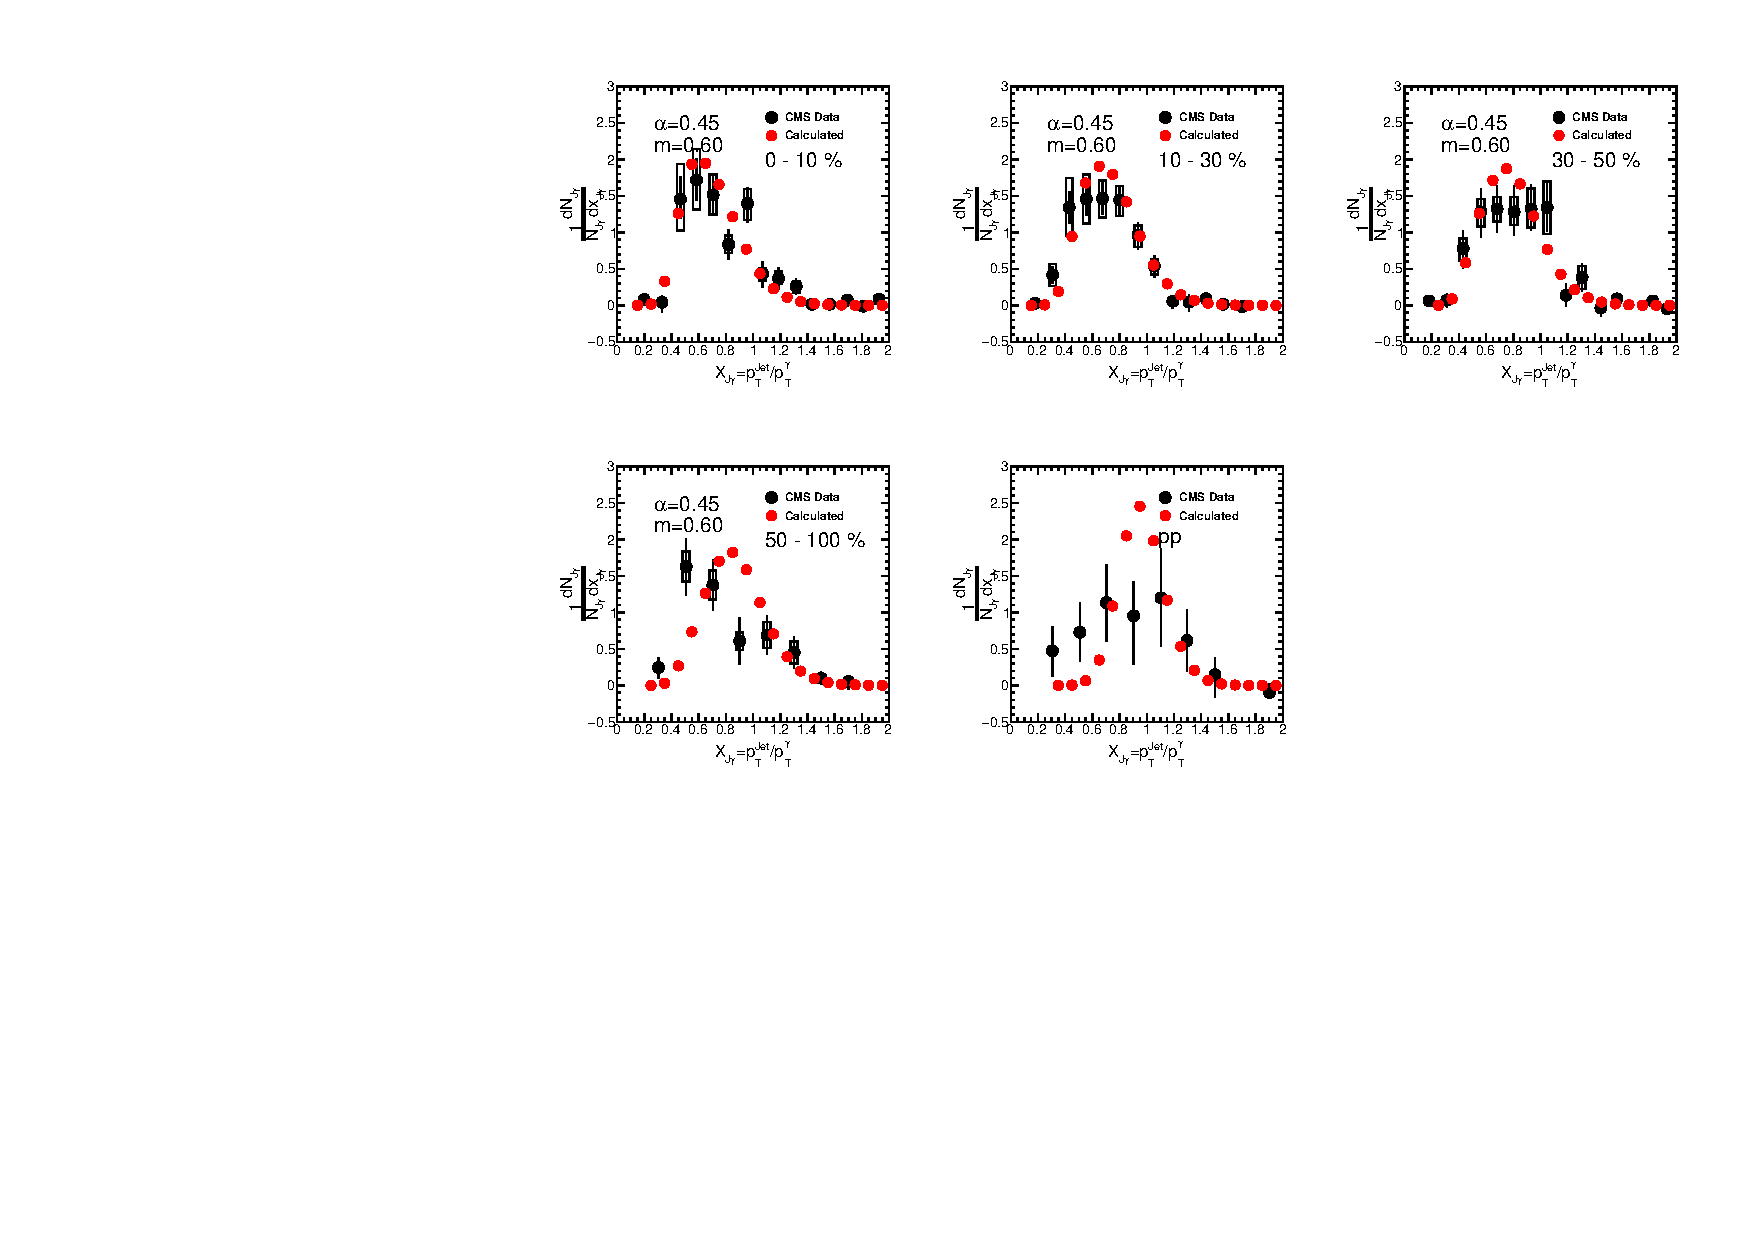
\includegraphics[width=0.99\textwidth]{Figures/Fig_XJ_GammaJet_Centrality.pdf}
  \caption{(Color online) Jet asymmatry as a function of collision centrality
    in gamma + Jet events as measured by CMS experiment. The data is compared with our
    calculations.}
  \label{Fig:JetAsymGammaJetCent}
\end{figure*}



\begin{figure*}
  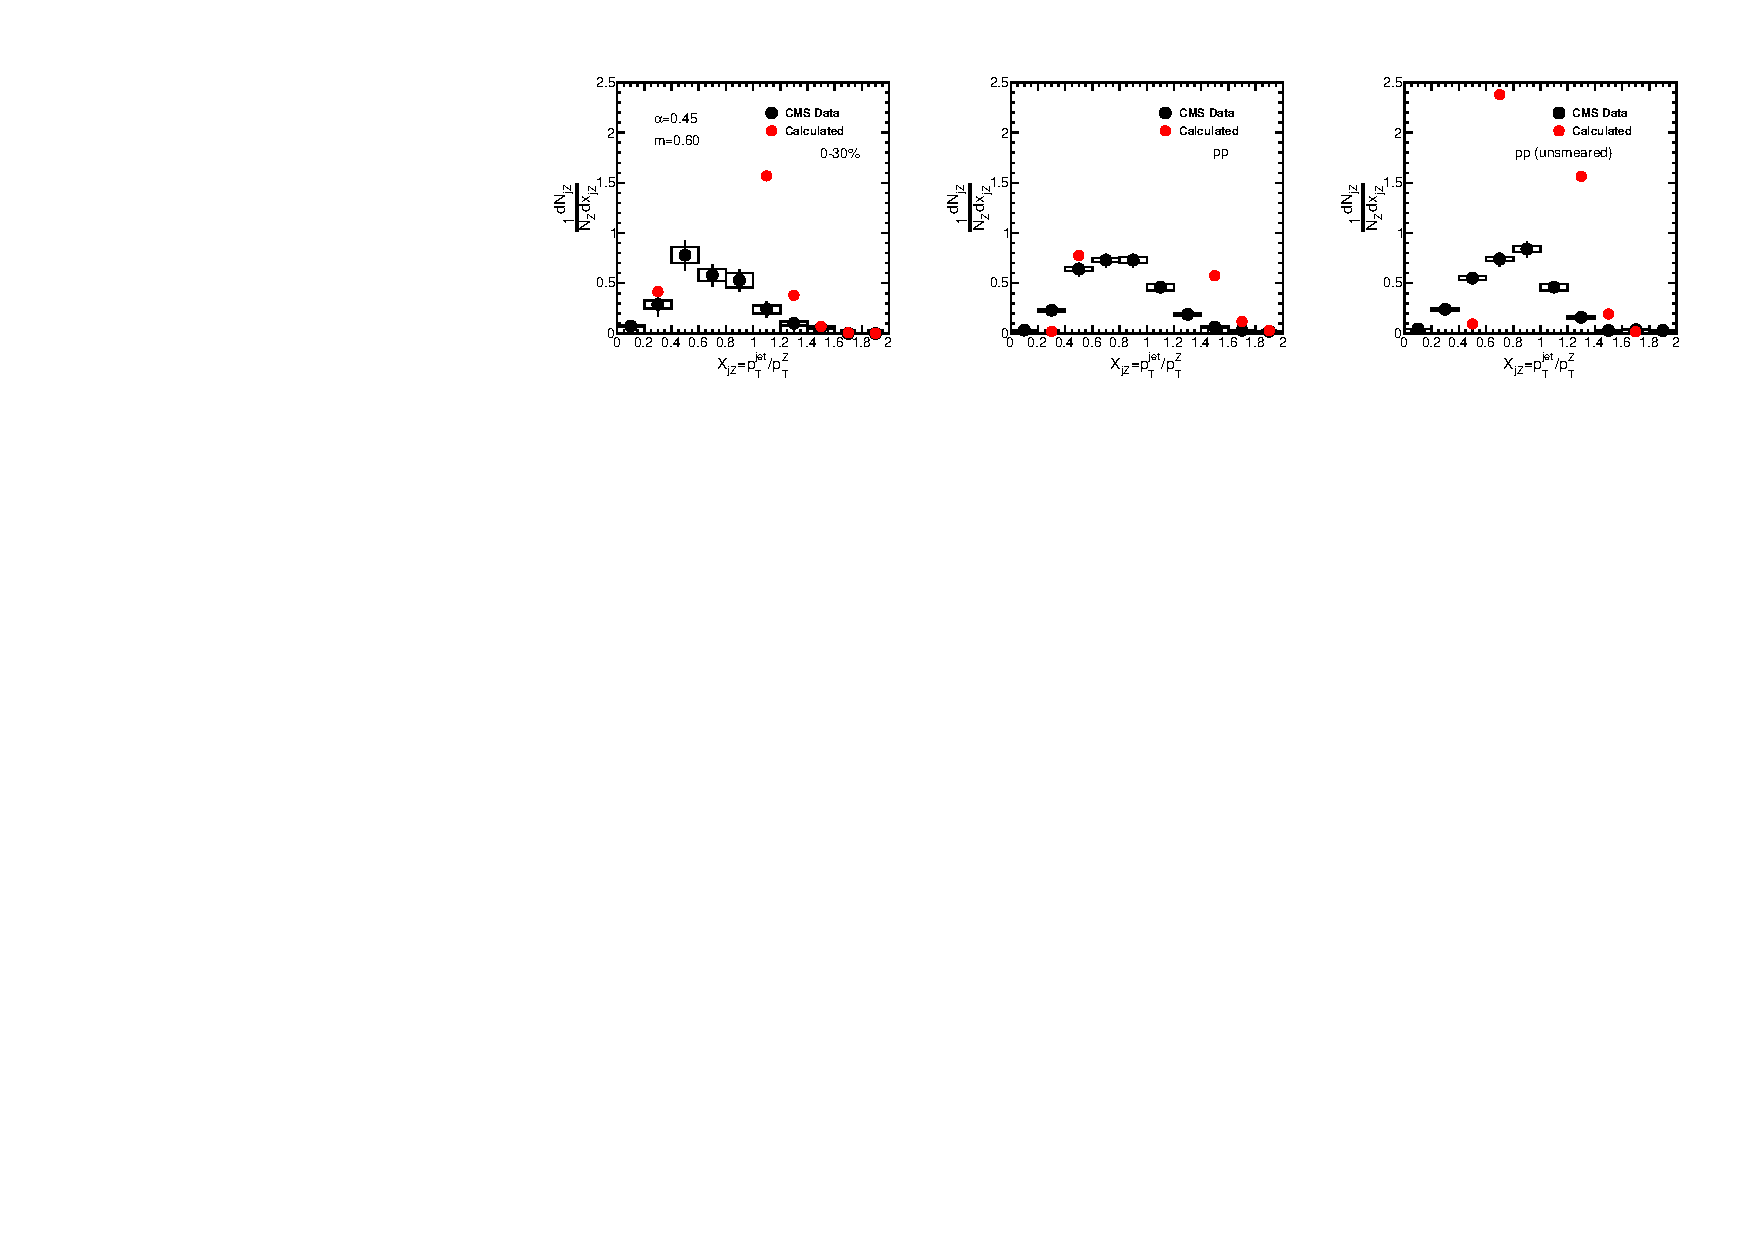
\includegraphics[width=0.99\textwidth]{Figures/Fig_XJ_Z0Jet_Centrality.pdf}
  \caption{(Color online) (Color online) Jet asymmatry as a function of collision centrality
    in Z$^{0}$ + Jet events as measured by CMS experiment. The data is compared with our
    calculations.}
  \label{Fig:JetAsymZ0JetCent}
\end{figure*}

\section{Results and discussions}
\label{Sec:ResultsAndDiss}


\section{Summary}
\label{Sec:Summary}



\begin{thebibliography}{100}
  
\bibitem{CUTS} J. SOllfrank, P. Huovinen, M. Kataja, P.V. Ruuskanen,
  M. Prakash and R. Venugopalan, 
  Phys. Rev. C{\bf 55}, 392 (1997).

\end{thebibliography}

\end{document}




